\documentclass[conference]{IEEEtran}
\IEEEoverridecommandlockouts
\usepackage{cite}
\usepackage{amsmath,amssymb,amsfonts}
\usepackage{algorithmic}
\usepackage{graphicx}
\usepackage{textcomp}
\usepackage{xcolor}
\def\BibTeX{{\rm B\kern-.05em{\sc i\kern-.025em b}\kern-.08em
    T\kern-.1667em\lower.7ex\hbox{E}\kern-.125emX}}
\begin{document}

\title{Idiolect: A Reconfigurable Voice Coding Assistant}

\author{\IEEEauthorblockN{Breandan Considine}
\IEEEauthorblockA{\textit{McGill University} \\
bre@ndan.co}
\and
\IEEEauthorblockN{Nicholas Albion}
\IEEEauthorblockA{\textit{Independent Developer} \\
nalbion@yahoo.com}
\and
\IEEEauthorblockN{Xujie Si}
\IEEEauthorblockA{\textit{University of Toronto} \\
xsi@cs.utoronto.ca}
}

\maketitle

\begin{abstract}
This paper presents Idiolect, an IDE plugin for voice coding and a novel approach to building bots that allows for users to define custom commands on-the-fly. Unlike traditional chatbots, Idiolect does not pretend to be an omnicient virtual assistant but rather a reconfigurable voice programming system that empowers users to create their own commands and actions dynamically, without rebuilding or restarting the application. We present a case study of integrating Idiolect~\footnote{https://github.com/OpenASR/idiolect} with the IntelliJ Platform, illustrate some example use cases, and offer some lessons learned during the tool's development.
\end{abstract}

\begin{IEEEkeywords}
    speech recognition, voice programming, bots
\end{IEEEkeywords}

\section{Introduction}


Humans are able to quickly learn new words and phrases, and apply them in a variety of contexts. Chatbots, on the other hand, are often limited to a set of static commands and phrases defined at compile-time. This can be frustrating for users, who struggle to express their intent, as well as bot-developers, who must anticipate user intent and write bindings for each new capability. This rigidity is a common source of misalignment between user intent, author expectations and bot capabilities.

%Considering  redefine commands addresses a common usability issue in voice UX design, where users are unable to express their intent in a way that the system understands. For example, a user may want to open a specific file, but the system only understands the command ``open file''. The user must then learn the system's command vocabulary, and then rephrase their intent in a way the system understands.
%On the other end of the spectrum are general-purpose scripting and metaprogramming languages that allow users to define their own commands and build embedded domain specific languages (eDSLs). These systems are highly flexible, but require a high upfront investment from the user, who must design a language to define their own commands, and then learn the language itself, all whilst doing their daily job as a software engineer.

Voice coding allows users to quickly dictate their own commands and phrases without resorting to a Turing Complete programming language. For example, the user might say ``whenever I say \textit{open sesame}, do the following action'', thereafter, the system will perform the desired action when so instructed. Or, ``whenever I say \textit{redo thrice}, repeat the last action three times''. Or, e.g., invoke a function in a scripting language, open a file, or perform other tedious chores.

Idiolect provides a default lexicon of phrases, but does not force users to learn them explicitly. Instead, we allow users to override the default settings with their own voice commands on-the-fly, which are incorporated into the lexicon immediately. This shifts the burden of adaptation to the system, freeing users to express their intent in a natural way.

Primarily, Idiolect observes the following design principles: be (1) natural to use, (2) easy to configure, (3) as unobtrusive as possible. We believe that these principles are important for a system intended to be used by developers, who are busy people and capable of configuring the system themselves. We also support developers with visual and motor impairments, who may have difficulty typing, or prefer to use a voice interface.

In this paper, we describe Idiolect, a dynamically reconfigurable system that allows users to teach the IDE new commands and actions on the fly, by either verbally or programmatically expressing the desired behavior.

%By targeting IDEs, whose users are already familiar with programming, commands that require complex instructions can be written programmatically, and then invoked on the fly with a keyword or phrase.

\section{Prior Work}

Mary Shaw, during her 2022 SPLASH keynote called for programming languages to address the needs of ``vernacular developers''. Jin Guo has also talked about the need for programming in ``ordinary people's langauge''. We take their proposals quite literally to mean that computers should be able to interpret spoken programs, and not just written ones.

Early attempts to build voice programming systems can be traced back at least twenty years to Leopold and Amber's (1997) work on keyboardless programming, later revisited by Arnold and Goldthwaite (2001), Begel and Graham's (2005) and others. These systems allow users to write code by speaking into a microphone, however early voice programming systems were limited by a small vocabulary, and do not consider IDE integration or reconfigurability.

Another stream of work has explored teaching voice assistants to use custom phrases (Chkroun \& Azaria, 2019). Their approach is similar to our own, but is limited to a single user, and does not consider more general forms of voice programming. It also predates most of the recent progress on large language modeling, which we consider to be a transformative enabling technology for this problem.

\section{Speech Models}

Today, automatic speech recognition (ASR), the translation of an audio waveform containing speech to text, is essentially a solved problem - one of the many pretrained ASR models would work well enough for our purposes. However, we also require realtime offline speech recognition capabilities built on an open source deep speech pipeline, which has only recently become possible for users running on commodity hardware.

Idiolect integrates with Vosk, a state-of-the-art deep speech system with realtime models for various languages, which provides an open source Java API. Initially, we distributed a default model for the English language inside the plugin, but at the request of JetBrains to reduce bandwidth, we instead prompt the user to select and download a pretrained model from the Vosk website upon first installing the plugin.

%For TTS, we use the built-in voices from the parent operating system, via the jAdapterForNativeTTS\footnote{https://github.com/jonelo/jAdapterForNativeTTS} library.

Users may optionally configure a built-in TTS voice from the host operating system and a cloud-based speech recognition or synthesis service, with the caveat that web speech requires uninterrupted internet connectivity and introduces an additional 300-500ms of overhead latency depending on the user's proximity to the datacenter and other load factors.

\section{Intent Recognition}

Once a spoken utterance is decoded as text, Idiolect must extract the relevant actions and entities to determine the user's intent. Furthermore, it may need to consider the IDE context, i.e., the current state of the editor and previous command history, to resolve potentially ambiguous commands. For example, the command ``open plugin menu'' could refer to multiple different menus, depending on when and how it was invoked.

The IntelliJ Platform has over $10^3$ possible actions. These actions are bound to keyboard shortcuts, menu items, and toolbar buttons. The user can also bind an action directly to voice commands, presuming the user already knows the action's identifier. Idiolect's default grammar was manually curated from the action list, using the CamelCase identifier to generate a suitable description for recognizing each intent.

Idiolect can match a user's utterance in a variety of ways, namely (1) lexical string matching, (2) context-free language recognition, and (3) LLM-prompting. By providing an extensible DSL, users can define their own command patterns via a simple configuration file, or programmatically using the plugin API to handle more complex usage scenarios.

In some cases, the user may not know or recall the exact phrase to which an action they intend to perform was bound. Given an utterance which does not match any of the predefined grammars, the plugin will fall back to a language model (LM), a probabilistic model trained on a large corpus of text, which can be used to perform reasoning simple tasks like predicting the most likely intent from a list of alternatives. For example, the utterance ``I want to edit foo.java'' is more likely to match the command ``open foo.java'' than ``execute foo.java''.

\subsection{Recognition Dispatch}

Idiolect dispatches utterances to a series of recognizers using a priority system. This system gives each recognizer the chance to match or pass on each utterance. Once a command is matched, the command is consumed and no subsequent recognizer will receive the dispatch.

The plugin first attempts to resolve a spoken utterance using an exact lexical match against a lexicon of predefined commands. Highest priority are those which control the plugin itself, enabling and disabling speech recognition.

User-defined commands are the next highest priority. These can be a lexical match, or more generally a sentence in a context-free language. Parsing parameters allows it to handle to more complex instructions, such as ``open the \textlangle filename\textrangle [in \textlangle project\_name\textrangle]'' or ``jump to the \textlangle nth\textrangle line''.

If there is no exact match, we attempt to repair the phrase using an error-correcting parser. We describe this in Sec.~\ref{sec:error}.

The recognizer of last resort is a large language model. Open ended commands which are unrecognizable by any of the previous approaches are dispatched to a service which matches the intent against a predefined lexicon. We can use a prompt, "What action is the most likely for the phrase "..." out of these actions: ..." and then delegate to the action choosen by the model.

\section{Error Recovery}\label{sec:error}

Idiolect supports defining and recognizing context-free and mildly context-sensitive grammars. In keeping with the design principle of configurability, we allow users to define custom grammars and bind phrases to actions. In many cases however, there are verbal fillers and extraneous text which cannot be parsed directly. When the utterance is one or two tokens away from a command, we attempt to repair the utternace using error recovery.

We address the issue of recognition errors by incorporating Considine et al.'s (2022) work on Tidyparse. In short, if a given phrase, e.g., ``open uh foo.java'' is uttered, we can repair the string to ``open foo.java''. Tidyparse implements a novel approach to error correction based on the theory of context-free language reachability, finite field arithmetic, conjunctive grammars and Levenshtein automata. We use a SAT solver to find the smallest edit transforming a string outside the language to a string inside the langauge.

Vosk is also capable of returning a list of alternate utterances, alongside a confidence score for each, which we use to determine if the user's utterance is sufficiently close to a known command.

Finally, we can use a language model to rerank the most likely utterances, conditioned on a previous context of historical commands. This is a form of error recovery, where we attempt to locate the most likely intent matching the user's utterance, given the dictionary, context and a list of alternate utterances.

\section{Large Langauge Models}

Recent progress in machine learning has enabled the use of large language models (LLMs) for a variety of tasks, including speech recognition, machine translation, and text generation. We can use an LLM to predict the most likely utterance given a sequence of words, for example, the utterance ``I want to edit foo.java'' is more likely to be the command ``open foo.java'' than the command ``execute foo.java''. While these models are currently served on the cloud, recent efforts to compress and do inference on commodity hardware are ongoing. We predict in the next few years these models will soon be available on the edge, and can be used to perform real-time intent recognition.

\section{User Onboarding}

Upon first installing the plugin, the user is greeted and prompted to download the Vosk model for recognizing their natural language of choice, which defaults to the system locale. Once unpacked, the model is stored in the plugin configuration directory, \texttt{~/.idealect}. The user is next prompted to configure the properties file, and to bind a few voice commands. This is a one-time process, and users may reconfigure the plugin by opening the settings dialog at any time.

\section{Plugin Extensions}

In addition to end-user configurability, Idiolect is designed to be extensible by external plugin developers and can be used by other IntelliJ Platform plugins to define their own commands. We provide a simple message passing API for plugins to communicate with Idiolect, and a DSL for defining custom commands.

\section{Build Automation}

To streamline the development process, we set up an automated pipeline for building and deploying the plugin. We use GitHub Actions to build the plugin for each release, and when a new commit is tagged with a release number and merged, a changelog is automatically generated from the intervening commit messages, then the plugin is signed and automatically uploaded to the JetBrains plugin repository. This allows us to quickly iterate on the plugin, test the plugin on multiple platforms, and to release new versions with minimal effort.

\section{Evaluation}

We evaluated the plugin on a variety of tasks. We also evaluated the plugin on tasks outside the default grammar, such as creating new projects, and running Gradle tasks. Our primary means of evaluation was user downloads of the plugin over a five-year timespan. We also performed a survey of users, to determine how satisfied they were with the plugin.

We then performed an intervention, by switching to a new voice recognition engine, and are collecting data on the number of downloads of the new version -- the results of this experiment are ongoing.

\section{Results}

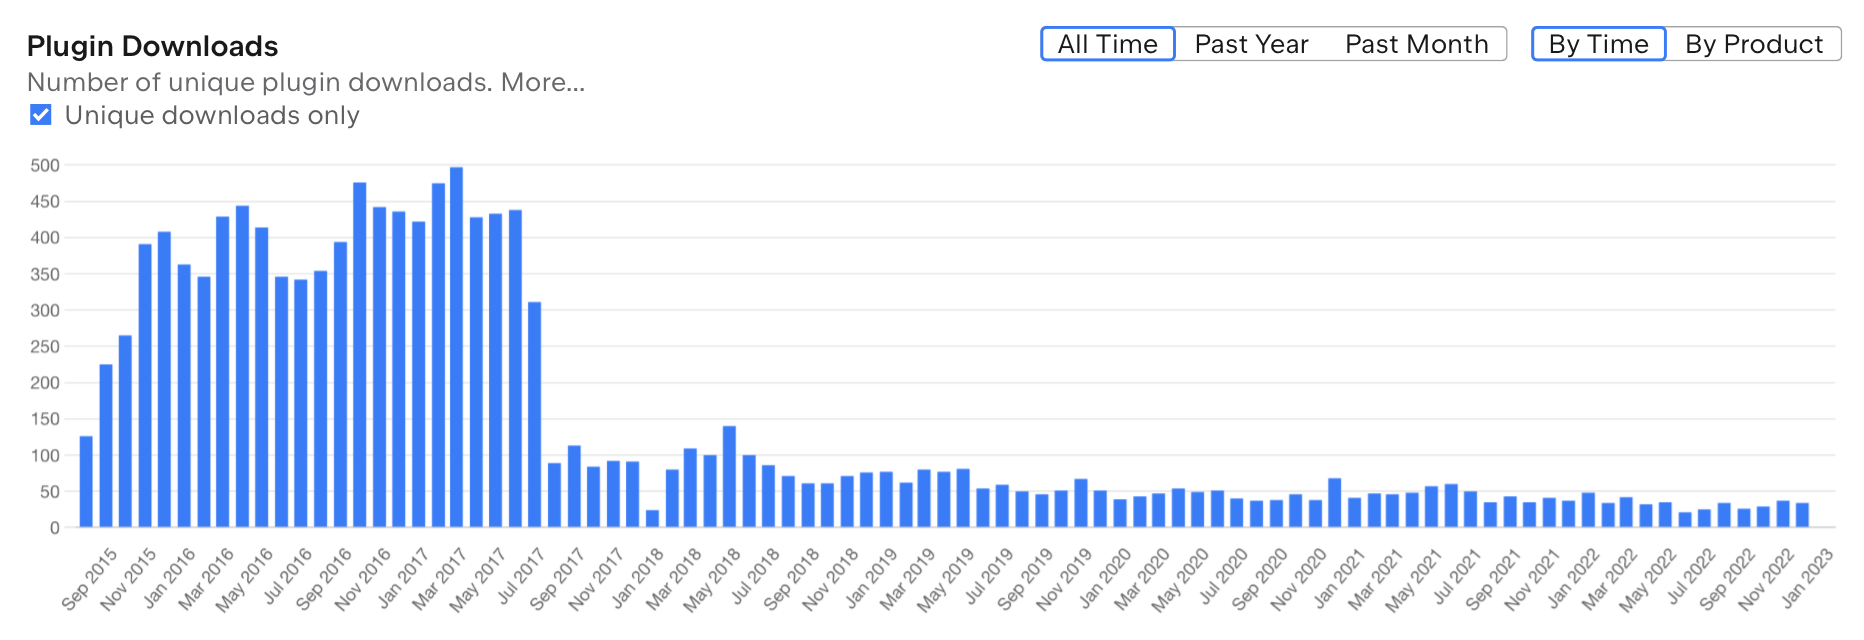
\includegraphics[width=0.45\textwidth]{downloads.png}

Downloads of the plugin have decreased over time since the plugin's initial release. We conjecture this relates to the fact that plugin was not updated for several years, and thus incompatible with the latest versions of IntelliJ Platform.

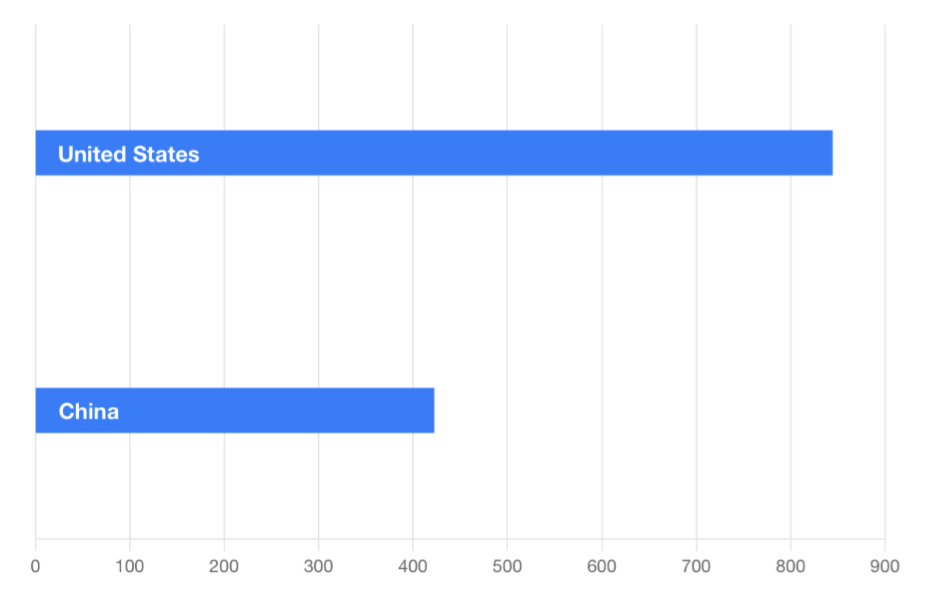
\includegraphics[width=0.50\textwidth]{demographics.png}

A careful inspection of demography indicates a large fraction of the plugin downloads originate from the People's Republic of China, indicating a substantial and potentially underserved programming demographic. A careful analysis suggests the need to support internationalization and localiation, an omission that we hope to remedy in a future release.

In addition, we performed an experiment to evaluate the performance of artificial speech recognition. Using a set of English TTS voices (male and female) included in MacOS Ventura 13.1, we synthesize a set of utterances from the predefined command list, feed them to VoskAPI, and evaluate the end-to-end intent recognition accuracy across two pretrained models: \texttt{vosk-model-small-en-us-0.15}, and \texttt{vosk-model-en-us-0.22-lgraph}. Results are shown in Table \ref{tab:results}.

\section{Future work}

In the future, we plan to conduct a thorough user study to better understand the use cases for the plugin. In particular, we hope to offer improved support for accessibility to facilitate the development habits of visually and motor-impaired users, as well as broader support for other languages and dialects.

We also aim to improve the interaction mechanism by adding audiovisual feedback and modes. A choose-your-adventure style modal dialog with a tree navigation mechanism, possibly integrating modal logical a la Hazel by adding a visual backpack and modal operators would be an interesting direction to take and one we hope to explore.

We also plan to conduct an evaluation of the plugin's intent-recognition capability and improve support for personalization, such as speaker adaptation and user-specific language models.

Finally we would like to provide a more user-friendly configuration interface, possibly using an embedded DSL for defining dialog trees.

To prioritize the development of these features, it would be helpful to collect telemetry to guide the development of the plugin and address the needs of voice programmers.

\section{Conclusion}

In this work, we presented Idiolect, a plugin for the IntelliJ Platform that allows users to control the IDE using voice commands. We described the design of the plugin, and the challenges we faced while implementing it. We also presented the results of our evaluation, and discussed future work.

\section{Acknowledgements}

The first author wishes to thank his former colleagues Alexey Kudinkin and Yaroslav Lepenkin, who contributed to the plugin during the original JetBrains hackathon in 2015, and former manager Hadi Hariri for his advice and encouragement.

\begin{thebibliography}{00}
\bibitem{b1} G. Eason, B. Noble, and I. N. Sneddon, ``On certain integrals of Lipschitz-Hankel type involving products of Bessel functions,'' Phil. Trans. Roy. Soc. London, vol. A247, pp. 529--551, April 1955.
\bibitem{b2} J. Clerk Maxwell, A Treatise on Electricity and Magnetism, 3rd ed., vol. 2. Oxford: Clarendon, 1892, pp.68--73.
\bibitem{b3} I. S. Jacobs and C. P. Bean, ``Fine particles, thin films and exchange anisotropy,'' in Magnetism, vol. III, G. T. Rado and H. Suhl, Eds. New York: Academic, 1963, pp. 271--350.
\bibitem{b4} K. Elissa, ``Title of paper if known,'' unpublished.
\bibitem{b5} R. Nicole, ``Title of paper with only first word capitalized,'' J. Name Stand. Abbrev., in press.
\end{thebibliography}
\end{document}
